\documentclass[11pt,a4paper]{article}

% Required packages
\usepackage[utf8]{inputenc}
\usepackage[T1]{fontenc}
\usepackage{amsmath}
\usepackage{amssymb}
\usepackage{amsfonts}
\usepackage{tikz}
\usepackage{geometry}
\usepackage{xcolor}

% TikZ libraries
\usetikzlibrary{positioning, arrows.meta, shapes.geometric, fit, backgrounds, shadows}

% Page geometry with smaller margins
\geometry{
    left=0.3cm,
    right=0.3cm,
    top=0.5cm,
    bottom=0.5cm
}

% Define custom colors
\definecolor{lightblue}{RGB}{173, 216, 230}
\definecolor{lightorange}{RGB}{255, 218, 185}
\definecolor{lightgreen}{RGB}{144, 238, 144}
\definecolor{lightyellow}{RGB}{255, 255, 224}
\definecolor{lightpink}{RGB}{255, 182, 193}
\definecolor{lightpurple}{RGB}{221, 160, 221}
\definecolor{mediumblue}{RGB}{135, 206, 235}
\definecolor{mediumgreen}{RGB}{152, 251, 152}
\definecolor{darkblue}{RGB}{70, 130, 180}
\definecolor{darkpurple}{RGB}{138, 43, 226}

% Compact TikZ styles
\tikzset{
    block/.style={
        rectangle, 
        draw, 
        thick, 
        rounded corners=4pt,
        minimum height=2.5cm, 
        minimum width=1.2cm,
        text width=1cm, 
        align=center, 
        font=\tiny\bfseries,
        inner sep=0.5pt,
        text depth=0pt,
        text height=0.2cm
    },
    toptextblock/.style={
        rectangle, 
        draw, 
        thick, 
        rounded corners=4pt,
        minimum height=2.5cm, 
        minimum width=1.2cm,
        text width=1cm, 
        align=center, 
        font=\tiny\bfseries,
        inner sep=0.5pt,
        text depth=0pt,
        text height=0.3cm
    },
    wideblock/.style={
        rectangle, 
        draw, 
        thick, 
        rounded corners=4pt,
        minimum height=2.5cm, 
        text width=1.8cm,
        align=center, 
        font=\tiny\bfseries,
        inner sep=0.2pt
    },
    smallblock/.style={
        rectangle, 
        draw, 
        thick, 
        rounded corners=3pt,
        minimum height=0.8cm, 
        text width=1.3cm, 
        align=center, 
        font=\scriptsize,
        inner sep=1pt
    },
    circleblock/.style={
        circle,
        draw,
        thick,
        minimum size=0.6cm,
        align=center,
        font=\scriptsize,
        inner sep=1pt
    },
    arrow/.style={-{Stealth[length=2mm, width=1.5mm]}, thick},
    dashedarrow/.style={-{Stealth[length=2mm, width=1.5mm]}, thick, dashed, red},
    estimatorbg/.style={
        fill=lightblue!20, 
        draw=darkblue, 
        rounded corners=6pt,
        inner sep=8pt
    },
    monitorbg/.style={
        fill=lightpurple!15, 
        draw=darkpurple, 
        rounded corners=6pt,
        inner sep=8pt
    }
}

\begin{document}

\begin{center}
\resizebox{\textwidth}{!}{%
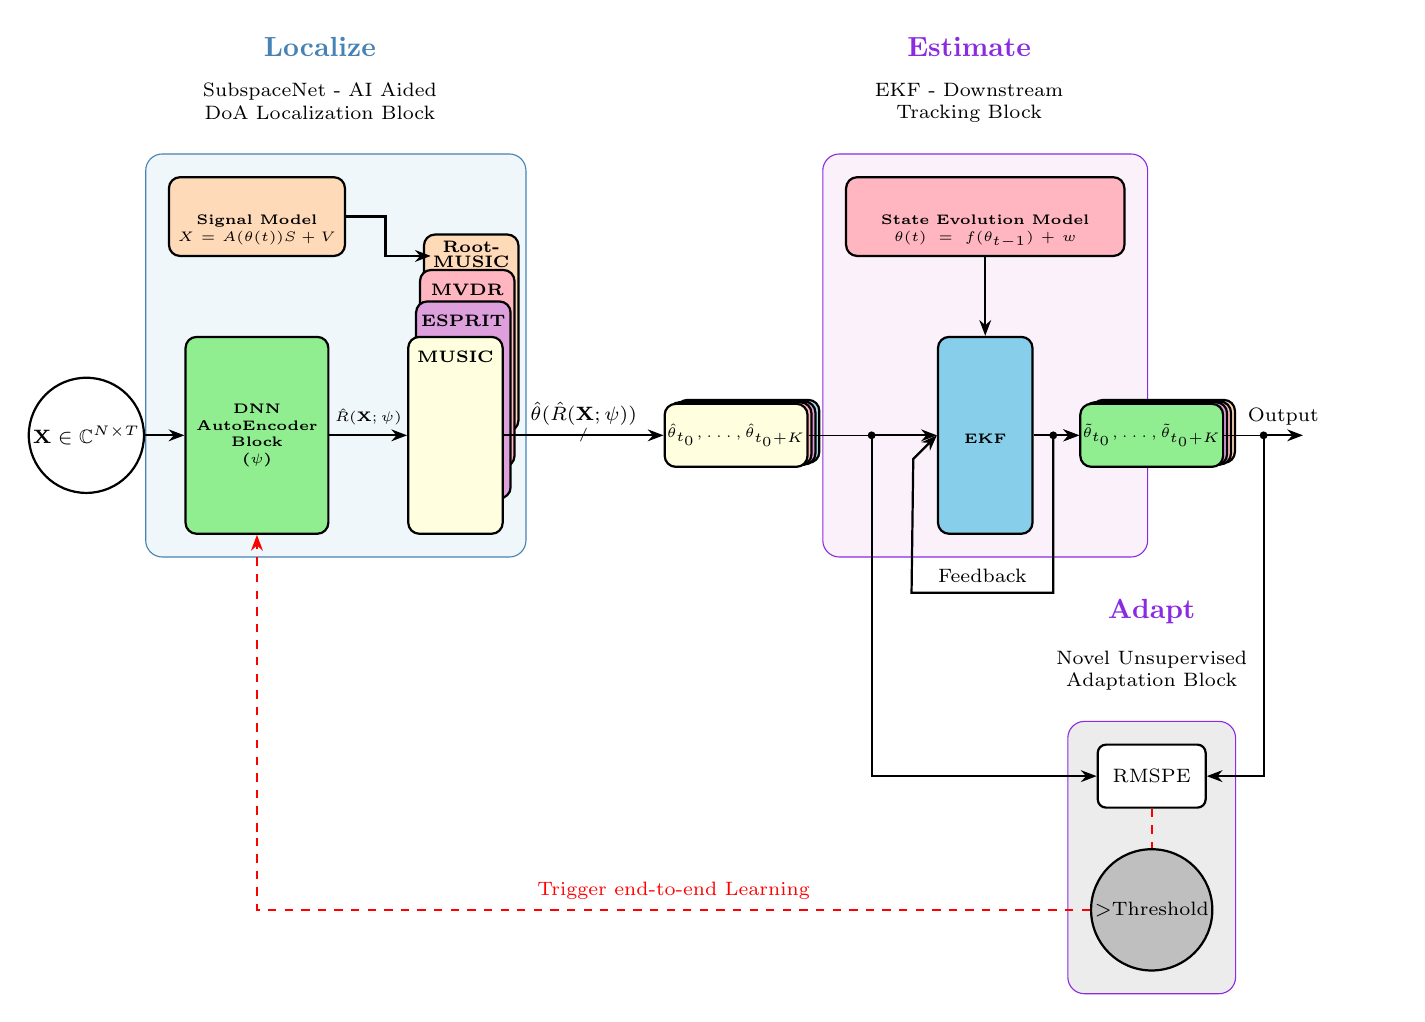
\begin{tikzpicture}[node distance=0.4cm]
    
    % Main processing chain - MERGED BLOCKS (removed rkhs block)
 \node[circleblock, fill=white] (input) at (-1,18) {$\mathbf{X} \in \mathbb{C}^{N \times T}$};
 \node[wideblock, fill=lightgreen, right=0.5cm of input] (dnn) {DNN\\AutoEncoder \\Block\\($\mathbf{\psi}$)};
 
     % Signal model input to DNN
    \node[block, fill=lightorange, above=1cm of dnn, text width=2.2cm, minimum height=1.0cm, align=center] (signal_model) {Signal Model\\$X=A(\theta(t))S+V$};
    
    
    % Estimator section title
    \node[font=\normalsize\bfseries, color=darkblue, above=1.4cm of signal_model, xshift=0.8cm] (est_title) {Localize};
    \node[font=\scriptsize, text width=4cm, align=center, below=0.1cm of est_title] (est_subtitle) {SubspaceNet - AI Aided \\DoA Localization Block};
    
    % Music stack (stacked blocks like folders)
    \coordinate (music_base) at ([xshift=1.6cm] dnn.east);
    \node[block, fill=lightorange, xshift=0.2cm, yshift=1.3cm] (music4) at (music_base) {};
    \node[font=\fontsize{6}{7}\selectfont\bfseries] at ([xshift=0.2cm, yshift=1.3cm, yshift=1.1cm] music_base) {Root-};
    \node[font=\fontsize{6}{7}\selectfont\bfseries] at ([xshift=0.2cm, yshift=1.3cm, yshift=0.9cm] music_base) {MUSIC};
    \node[block, fill=lightpink, xshift=0.15cm, yshift=0.85cm] (music3) at (music_base) {};
    \node[font=\fontsize{6}{7}\selectfont\bfseries] at ([xshift=0.15cm, yshift=0.85cm, yshift=1.0cm] music_base) {MVDR};
    \node[block, fill=lightpurple, xshift=0.1cm, yshift=0.45cm] (music2) at (music_base) {};
    \node[font=\fontsize{6}{7}\selectfont\bfseries] at ([xshift=0.1cm, yshift=0.45cm, yshift=1.0cm] music_base) {ESPRIT};
    \node[block, fill=lightyellow] (music1) at (music_base) {};
    \node[font=\fontsize{6}{7}\selectfont\bfseries] at ([yshift=1.0cm] music_base) {MUSIC};
    
    % Theta hat cascade (stacked blocks like folders)
    \coordinate (theta_base) at ([xshift=2.95cm] music1.east);
    \node[wideblock, fill=lightblue, xshift=0.15cm, yshift=0.05cm, minimum height=0.8cm] (theta4) at (theta_base) {};
    \node[wideblock, fill=lightpurple, xshift=0.1cm, yshift=0.03cm, minimum height=0.8cm] (theta3) at (theta_base) {};
    \node[wideblock, fill=lightpink, xshift=0.05cm, yshift=0.02cm, minimum height=0.8cm] (theta2) at (theta_base) {};
    \node[wideblock, fill=lightyellow, minimum height=0.8cm] (new_block) at (theta_base) {$\hat{\theta}_{t_0},\ldots,\hat{\theta}_{t_0+K}$};
    
    % Monitor section
    \node[font=\normalsize\bfseries, color=darkpurple, right=6.5cm of est_title] (mon_title) {Estimate};
    \node[font=\scriptsize, text width=6cm, align=center, below=0.1cm of mon_title] (mon_subtitle) {EKF - Downstream \\Tracking Block};
    
    % Monitor components
    \node[block, fill=mediumblue, right=5.5cm of music1] (kalman) {EKF};
    
    % State evolution model input to EKF
    \node[block, fill=lightpink, above=1cm of kalman, text width=3.5cm, minimum height=1.0cm, align=center] (state_model) {State Evolution Model\\$\theta(t) = f(\theta_{t-1})+w$};
    
    % Theta wave cascade (stacked blocks like folders)
    \coordinate (wave_base) at ([xshift=1.5cm] kalman.east);
    \node[wideblock, fill=lightorange, xshift=0.15cm, yshift=0.05cm, minimum height=0.8cm] (wave4) at (wave_base) {};
    \node[wideblock, fill=lightpink, xshift=0.1cm, yshift=0.03cm, minimum height=0.8cm] (wave3) at (wave_base) {};
    \node[wideblock, fill=lightpurple, xshift=0.05cm, yshift=0.02cm, minimum height=0.8cm] (wave2) at (wave_base) {};
    \node[wideblock, fill=lightgreen, minimum height=0.8cm] (output) at (wave_base) {$\tilde{\theta}_{t_0},\ldots,\tilde{\theta}_{t_0+K}$};
    
    % RMSPE block (inside monitor)
    \node[smallblock, fill=white, below=3.5cm of output] (minus) {RMSPE};
    
    % Adapt section title
    \node[font=\normalsize\bfseries, color=darkpurple, above=1.4cm of minus] (adapt_title) {Adapt};
    \node[font=\scriptsize, text width=6cm, align=center, below=0.1cm of adapt_title] (adapt_subtitle) {Novel Unsupervised \\Adaptation Block};
    % Threshold circle block
    \node[circleblock, fill=lightgray, below=0.5cm of minus] (threshold) {$>$Threshold};

    
    % Background regions (removed rkhs from estimator fit)
    \begin{scope}[on background layer]
        \node[estimatorbg, fit=(dnn)(music1)(signal_model)] {};
        \node[monitorbg, fit=(kalman)(state_model)] {};
        \node[monitorbg, fill=lightgray!30, fit=(minus)(threshold)] {};
    \end{scope}
    
    % Main flow arrows (direct connection from dnn to music1 with R hat label)
    \draw[arrow] (input) -- (dnn);
    \coordinate (signal_right) at ([xshift=0.5cm] signal_model.east);
 \coordinate (signal_down) at ([yshift=-0.5cm] signal_right);
 \coordinate (signal_final) at ([xshift=0.1cm] music4.west |- signal_down);
 \draw[arrow] (signal_model) -- (signal_right) -- (signal_down) -- (signal_final);
    \draw[arrow] (dnn) -- (music1) node[midway, above, font=\tiny] {$\hat{R}(\mathbf{X}; \mathbf{\psi})$};
    
    % Monitor connections
    \draw[arrow] (music1) -- (new_block) node[midway, above, font=\scriptsize] {$\hat{\theta}(\hat{R}(\mathbf{X}; \mathbf{\psi}))$} node[midway, sloped, font=\tiny] {/};
    
    % Split point for theta hat to EKF connection
    \coordinate (theta_split) at ([xshift=0.8cm] new_block.east);
    \node[circle, fill=black, minimum size=0.1cm, inner sep=0pt] at (theta_split) {};
    \draw (new_block) -- (theta_split);
    \draw[arrow] (theta_split) -- (kalman);
    \draw[arrow] (theta_split) |- (minus);
    
    \draw[arrow] (state_model) -- (kalman);
    \draw[arrow] (kalman) -- (output);
    
    % Split point for feedback loop from EKF to theta wave cascade (middle of arrow)
    \coordinate (feedback_split) at ([xshift=0.25cm] kalman.east);
    \node[circle, fill=black, minimum size=0.1cm, inner sep=0pt] at (feedback_split) {};
    \draw (kalman) -- (feedback_split);
    \draw[arrow] (feedback_split) -- (output);
    
    % Feedback loop (4 points: split-down-left-up-connection to below kalman.west)
    \coordinate (fb_down_point) at ([yshift=-2cm] feedback_split);
    \coordinate (fb_left_point) at ([xshift=-1.8cm] fb_down_point);
    \coordinate (fb_up_point) at ([yshift=-0.3cm, xshift=-0.3cm] kalman.west);
    \draw[arrow] (feedback_split) -- (fb_down_point) -- (fb_left_point) node[midway, above, font=\scriptsize] {Feedback} -- (fb_up_point) -- (kalman.west);
    
    % Split point for output arrow
    \coordinate (output_split) at ([xshift=0.5cm] output.east);
    \node[circle, fill=black, minimum size=0.1cm, inner sep=0pt] at (output_split) {};
    \draw (output) -- (output_split);
    \draw[arrow] (output_split) -- ([xshift=1cm] output.east) node[midway, above, font=\scriptsize] {Output};
    \draw[arrow] (output_split) |- (minus);
    
    
    % Output from minus block to DNN through threshold (left->up) - Learning Trigger
    \coordinate (intermediate1) at ([xshift=-11.36cm] threshold);
    \coordinate (intermediate2) at ([yshift=1cm] intermediate1);
    \draw[thick, dashed, red] (minus) -- (threshold);
    \draw[thick, dashed, red] (threshold) -- (intermediate1) node[midway, above, font=\scriptsize, red] {Trigger end-to-end Learning} -- (intermediate2);
    \draw[dashedarrow] (intermediate2) -| (dnn);
    
\end{tikzpicture}%
}
\end{center}

\end{document}